\documentclass[12pt,]{article}
\usepackage{lmodern}
\usepackage{amssymb,amsmath}
\usepackage{ifxetex,ifluatex}
\usepackage{fixltx2e} % provides \textsubscript
\ifnum 0\ifxetex 1\fi\ifluatex 1\fi=0 % if pdftex
  \usepackage[T1]{fontenc}
  \usepackage[utf8]{inputenc}
\else % if luatex or xelatex
  \ifxetex
    \usepackage{mathspec}
  \else
    \usepackage{fontspec}
  \fi
  \defaultfontfeatures{Ligatures=TeX,Scale=MatchLowercase}
    \setmainfont[]{Times New Roman}
\fi
% use upquote if available, for straight quotes in verbatim environments
\IfFileExists{upquote.sty}{\usepackage{upquote}}{}
% use microtype if available
\IfFileExists{microtype.sty}{%
\usepackage{microtype}
\UseMicrotypeSet[protrusion]{basicmath} % disable protrusion for tt fonts
}{}
\usepackage[margin=2.54cm]{geometry}
\usepackage{hyperref}
\hypersetup{unicode=true,
            pdftitle={Experiment Title},
            pdfauthor={Your Name},
            pdfborder={0 0 0},
            breaklinks=true}
\urlstyle{same}  % don't use monospace font for urls
\usepackage{color}
\usepackage{fancyvrb}
\newcommand{\VerbBar}{|}
\newcommand{\VERB}{\Verb[commandchars=\\\{\}]}
\DefineVerbatimEnvironment{Highlighting}{Verbatim}{commandchars=\\\{\}}
% Add ',fontsize=\small' for more characters per line
\usepackage{framed}
\definecolor{shadecolor}{RGB}{248,248,248}
\newenvironment{Shaded}{\begin{snugshade}}{\end{snugshade}}
\newcommand{\KeywordTok}[1]{\textcolor[rgb]{0.13,0.29,0.53}{\textbf{#1}}}
\newcommand{\DataTypeTok}[1]{\textcolor[rgb]{0.13,0.29,0.53}{#1}}
\newcommand{\DecValTok}[1]{\textcolor[rgb]{0.00,0.00,0.81}{#1}}
\newcommand{\BaseNTok}[1]{\textcolor[rgb]{0.00,0.00,0.81}{#1}}
\newcommand{\FloatTok}[1]{\textcolor[rgb]{0.00,0.00,0.81}{#1}}
\newcommand{\ConstantTok}[1]{\textcolor[rgb]{0.00,0.00,0.00}{#1}}
\newcommand{\CharTok}[1]{\textcolor[rgb]{0.31,0.60,0.02}{#1}}
\newcommand{\SpecialCharTok}[1]{\textcolor[rgb]{0.00,0.00,0.00}{#1}}
\newcommand{\StringTok}[1]{\textcolor[rgb]{0.31,0.60,0.02}{#1}}
\newcommand{\VerbatimStringTok}[1]{\textcolor[rgb]{0.31,0.60,0.02}{#1}}
\newcommand{\SpecialStringTok}[1]{\textcolor[rgb]{0.31,0.60,0.02}{#1}}
\newcommand{\ImportTok}[1]{#1}
\newcommand{\CommentTok}[1]{\textcolor[rgb]{0.56,0.35,0.01}{\textit{#1}}}
\newcommand{\DocumentationTok}[1]{\textcolor[rgb]{0.56,0.35,0.01}{\textbf{\textit{#1}}}}
\newcommand{\AnnotationTok}[1]{\textcolor[rgb]{0.56,0.35,0.01}{\textbf{\textit{#1}}}}
\newcommand{\CommentVarTok}[1]{\textcolor[rgb]{0.56,0.35,0.01}{\textbf{\textit{#1}}}}
\newcommand{\OtherTok}[1]{\textcolor[rgb]{0.56,0.35,0.01}{#1}}
\newcommand{\FunctionTok}[1]{\textcolor[rgb]{0.00,0.00,0.00}{#1}}
\newcommand{\VariableTok}[1]{\textcolor[rgb]{0.00,0.00,0.00}{#1}}
\newcommand{\ControlFlowTok}[1]{\textcolor[rgb]{0.13,0.29,0.53}{\textbf{#1}}}
\newcommand{\OperatorTok}[1]{\textcolor[rgb]{0.81,0.36,0.00}{\textbf{#1}}}
\newcommand{\BuiltInTok}[1]{#1}
\newcommand{\ExtensionTok}[1]{#1}
\newcommand{\PreprocessorTok}[1]{\textcolor[rgb]{0.56,0.35,0.01}{\textit{#1}}}
\newcommand{\AttributeTok}[1]{\textcolor[rgb]{0.77,0.63,0.00}{#1}}
\newcommand{\RegionMarkerTok}[1]{#1}
\newcommand{\InformationTok}[1]{\textcolor[rgb]{0.56,0.35,0.01}{\textbf{\textit{#1}}}}
\newcommand{\WarningTok}[1]{\textcolor[rgb]{0.56,0.35,0.01}{\textbf{\textit{#1}}}}
\newcommand{\AlertTok}[1]{\textcolor[rgb]{0.94,0.16,0.16}{#1}}
\newcommand{\ErrorTok}[1]{\textcolor[rgb]{0.64,0.00,0.00}{\textbf{#1}}}
\newcommand{\NormalTok}[1]{#1}
\usepackage{graphicx,grffile}
\makeatletter
\def\maxwidth{\ifdim\Gin@nat@width>\linewidth\linewidth\else\Gin@nat@width\fi}
\def\maxheight{\ifdim\Gin@nat@height>\textheight\textheight\else\Gin@nat@height\fi}
\makeatother
% Scale images if necessary, so that they will not overflow the page
% margins by default, and it is still possible to overwrite the defaults
% using explicit options in \includegraphics[width, height, ...]{}
\setkeys{Gin}{width=\maxwidth,height=\maxheight,keepaspectratio}
\IfFileExists{parskip.sty}{%
\usepackage{parskip}
}{% else
\setlength{\parindent}{0pt}
\setlength{\parskip}{6pt plus 2pt minus 1pt}
}
\setlength{\emergencystretch}{3em}  % prevent overfull lines
\providecommand{\tightlist}{%
  \setlength{\itemsep}{0pt}\setlength{\parskip}{0pt}}
\setcounter{secnumdepth}{5}
% Redefines (sub)paragraphs to behave more like sections
\ifx\paragraph\undefined\else
\let\oldparagraph\paragraph
\renewcommand{\paragraph}[1]{\oldparagraph{#1}\mbox{}}
\fi
\ifx\subparagraph\undefined\else
\let\oldsubparagraph\subparagraph
\renewcommand{\subparagraph}[1]{\oldsubparagraph{#1}\mbox{}}
\fi

%%% Use protect on footnotes to avoid problems with footnotes in titles
\let\rmarkdownfootnote\footnote%
\def\footnote{\protect\rmarkdownfootnote}

%%% Change title format to be more compact
\usepackage{titling}

% Create subtitle command for use in maketitle
\providecommand{\subtitle}[1]{
  \posttitle{
    \begin{center}\large#1\end{center}
    }
}

\setlength{\droptitle}{-2em}

  \title{Experiment Title}
    \pretitle{\vspace{\droptitle}\centering\huge}
  \posttitle{\par}
  \subtitle{Web address for GitHub repository}
  \author{Your Name}
    \preauthor{\centering\large\emph}
  \postauthor{\par}
    \date{}
    \predate{}\postdate{}
  

\begin{document}
\maketitle
\begin{abstract}
Experimental overview. This section should be no longer than 250 words.
\end{abstract}

\newpage

\tableofcontents  \newpage
\listoftables  \newpage
\listoffigures  \newpage

\textless{}Note: set up autoreferencing for figures and tables in your
document\textgreater{}

\section{Research Question and
Rationale}\label{research-question-and-rationale}

\newpage

\section{Dataset Information}\label{dataset-information}

\newpage

\section{Exploratory Data Analysis and
Wrangling}\label{exploratory-data-analysis-and-wrangling}

\begin{Shaded}
\begin{Highlighting}[]
\NormalTok{World_Bank_Master <-}\KeywordTok{read.csv}\NormalTok{(}\StringTok{"../Raw/WorldBank_Raw2_4.8.19.csv"}\NormalTok{)}

\CommentTok{#Data Subset}
\NormalTok{World_Bank_Filter <-}\StringTok{ }\KeywordTok{filter}\NormalTok{(World_Bank_Master, Indicator.Name }\OperatorTok{==}\StringTok{ "Forest area (% of land area)"} \OperatorTok{|}\StringTok{ }\NormalTok{Indicator.Name }\OperatorTok{==}\StringTok{ "Agricultural land (% of land area)"} \OperatorTok{|}\StringTok{ }\NormalTok{Indicator.Name }\OperatorTok{==}\StringTok{ "Arable land (% of land area)"} \OperatorTok{|}\StringTok{ }\NormalTok{Indicator.Name }\OperatorTok{==}\StringTok{ "Access to electricity (% of population)"} \OperatorTok{|}\StringTok{ }\NormalTok{Indicator.Name }\OperatorTok{==}\StringTok{ "Renewable electricity output (% of total electricity output)"} \OperatorTok{|}\StringTok{ }\NormalTok{Indicator.Name }\OperatorTok{==}\StringTok{ "CO2 emissions (kt)"} \OperatorTok{|}\StringTok{ }\NormalTok{Indicator.Name }\OperatorTok{==}\StringTok{ "Agricultural nitrous oxide emissions (thousand metric tons of CO2 equivalent)"} \OperatorTok{|}\StringTok{ }\NormalTok{Indicator.Name }\OperatorTok{==}\StringTok{ "Agricultural methane emissions (thousand metric tons of CO2 equivalent)"} \OperatorTok{|}\StringTok{ }\NormalTok{Indicator.Name }\OperatorTok{==}\StringTok{ "Aquaculture production (metric tons)"}\NormalTok{)}

\NormalTok{WorldBank_Gather <-}\StringTok{ }\KeywordTok{gather}\NormalTok{(World_Bank_Filter, }\StringTok{"Year"}\NormalTok{, }\StringTok{"Level"}\NormalTok{, X1960}\OperatorTok{:}\NormalTok{X2018)}

\NormalTok{WorldBank_Gather <-}\StringTok{ }\KeywordTok{select}\NormalTok{(WorldBank_Gather, }\OperatorTok{-}\NormalTok{Indicator.Code)}

\NormalTok{WorldBank_Spread <-}\StringTok{  }\KeywordTok{spread}\NormalTok{(WorldBank_Gather, Indicator.Name, Level)}

\CommentTok{#Format as character }
\NormalTok{WorldBank_Spread}\OperatorTok{$}\NormalTok{Year <-}\StringTok{ }\KeywordTok{as.character}\NormalTok{(WorldBank_Spread}\OperatorTok{$}\NormalTok{Year)}

\CommentTok{#create string}
\NormalTok{WB_String <-}\StringTok{ }\KeywordTok{substr}\NormalTok{(WorldBank_Spread}\OperatorTok{$}\NormalTok{Year, }\DecValTok{2}\NormalTok{, }\DecValTok{5}\NormalTok{)}

\CommentTok{#Get rid of X in date}
\NormalTok{WorldBank_Spread}\OperatorTok{$}\NormalTok{Year =}\StringTok{ }\NormalTok{WB_String}

\CommentTok{#Format as date}
\CommentTok{#WB_Fixed$Year <- as.Date(WB_Fixed$Year)}
\NormalTok{WorldBank_Spread}\OperatorTok{$}\NormalTok{Year <-}\StringTok{ }\KeywordTok{as.Date}\NormalTok{(WorldBank_Spread}\OperatorTok{$}\NormalTok{Year, }\DataTypeTok{format =} \StringTok{"%Y"}\NormalTok{) }\CommentTok{#can I get it to show only the year? }

\KeywordTok{class}\NormalTok{(WorldBank_Spread}\OperatorTok{$}\NormalTok{Year)}
\end{Highlighting}
\end{Shaded}

\begin{verbatim}
## [1] "Date"
\end{verbatim}

\begin{Shaded}
\begin{Highlighting}[]
\CommentTok{#Change column names }
\KeywordTok{names}\NormalTok{(WorldBank_Spread) <-}\StringTok{ }\KeywordTok{c}\NormalTok{(}\StringTok{"Country"}\NormalTok{, }\StringTok{"Indicator.Code"}\NormalTok{, }\StringTok{"Year"}\NormalTok{, }\StringTok{"Electricity Access"}\NormalTok{, }\StringTok{"Agriculture"}\NormalTok{, }\StringTok{"Ag.Methane"}\NormalTok{, }\StringTok{"Ag.NO2"}\NormalTok{, }\StringTok{"Aquaculture"}\NormalTok{, }\StringTok{"ArableLand"}\NormalTok{, }\StringTok{"CO2Emissions"}\NormalTok{, }\StringTok{"Forest"}\NormalTok{, }\StringTok{"RenewableElectricity"}\NormalTok{)}

\CommentTok{#Save processed file }
\CommentTok{#write.csv(WorldBank_Spread, row.names = FALSE, file = "../Processed/WorldBank_Processed.csv")}
   
\NormalTok{Four_Countries <-}\StringTok{ }\KeywordTok{filter}\NormalTok{(WorldBank_Spread, Country }\OperatorTok{==}\StringTok{ "Brazil"} \OperatorTok{|}\StringTok{ }\NormalTok{Country }\OperatorTok{==}\StringTok{ "Spain"} \OperatorTok{|}\StringTok{ }\NormalTok{Country }\OperatorTok{==}\StringTok{ "Indonesia"} \OperatorTok{|}\StringTok{ }\NormalTok{Country }\OperatorTok{==}\StringTok{ "Canada"}\NormalTok{)}

\NormalTok{Five_Countries <-}\StringTok{ }\KeywordTok{filter}\NormalTok{(WorldBank_Spread, Country }\OperatorTok{==}\StringTok{ "Brazil"} \OperatorTok{|}\StringTok{ }\NormalTok{Country }\OperatorTok{==}\StringTok{ "Kenya"} \OperatorTok{|}\StringTok{ }\NormalTok{Country }\OperatorTok{==}\StringTok{ "Spain"} \OperatorTok{|}\StringTok{ }\NormalTok{Country }\OperatorTok{==}\StringTok{ "Indonesia"} \OperatorTok{|}\StringTok{ }\NormalTok{Country }\OperatorTok{==}\StringTok{ "Canada"}\NormalTok{)}

\NormalTok{Six_Countries <-}\StringTok{ }\KeywordTok{filter}\NormalTok{(WorldBank_Spread, Country }\OperatorTok{==}\StringTok{ "Brazil"} \OperatorTok{|}\StringTok{ }\NormalTok{Country }\OperatorTok{==}\StringTok{ "Kenya"} \OperatorTok{|}\StringTok{ }\NormalTok{Country }\OperatorTok{==}\StringTok{ "Spain"} \OperatorTok{|}\StringTok{ }\NormalTok{Country }\OperatorTok{==}\StringTok{ "Pakistan"} \OperatorTok{|}\StringTok{ }\NormalTok{Country }\OperatorTok{==}\StringTok{ "Indonesia"} \OperatorTok{|}\StringTok{ }\NormalTok{Country }\OperatorTok{==}\StringTok{ "Canada"}\NormalTok{)}
\end{Highlighting}
\end{Shaded}

\begin{Shaded}
\begin{Highlighting}[]
\KeywordTok{colnames}\NormalTok{(WorldBank_Spread)}
\end{Highlighting}
\end{Shaded}

\begin{verbatim}
##  [1] "Country"              "Indicator.Code"       "Year"                
##  [4] "Electricity Access"   "Agriculture"          "Ag.Methane"          
##  [7] "Ag.NO2"               "Aquaculture"          "ArableLand"          
## [10] "CO2Emissions"         "Forest"               "RenewableElectricity"
\end{verbatim}

\begin{Shaded}
\begin{Highlighting}[]
\KeywordTok{dim}\NormalTok{(WorldBank_Spread)}
\end{Highlighting}
\end{Shaded}

\begin{verbatim}
## [1] 15576    12
\end{verbatim}

\begin{Shaded}
\begin{Highlighting}[]
\KeywordTok{head}\NormalTok{(WorldBank_Spread)}
\end{Highlighting}
\end{Shaded}

\begin{verbatim}
##       Country Indicator.Code       Year Electricity Access Agriculture
## 1 Afghanistan            AFG 1960-04-10                 NA          NA
## 2 Afghanistan            AFG 1961-04-10                 NA    57.74592
## 3 Afghanistan            AFG 1962-04-10                 NA    57.83782
## 4 Afghanistan            AFG 1963-04-10                 NA    57.91441
## 5 Afghanistan            AFG 1964-04-10                 NA    58.01091
## 6 Afghanistan            AFG 1965-04-10                 NA    58.01397
##   Ag.Methane Ag.NO2 Aquaculture ArableLand CO2Emissions Forest
## 1         NA     NA          NA         NA      414.371     NA
## 2         NA     NA          NA   11.71767      491.378     NA
## 3         NA     NA          NA   11.79426      689.396     NA
## 4         NA     NA          NA   11.87085      707.731     NA
## 5         NA     NA          NA   11.94743      839.743     NA
## 6         NA     NA          NA   11.94743     1008.425     NA
##   RenewableElectricity
## 1                   NA
## 2                   NA
## 3                   NA
## 4                   NA
## 5                   NA
## 6                   NA
\end{verbatim}

\begin{Shaded}
\begin{Highlighting}[]
\KeywordTok{summary}\NormalTok{(WorldBank_Spread)}
\end{Highlighting}
\end{Shaded}

\begin{verbatim}
##            Country      Indicator.Code       Year           
##  Afghanistan   :   59   ABW    :   59   Min.   :1960-04-10  
##  Albania       :   59   AFG    :   59   1st Qu.:1974-04-10  
##  Algeria       :   59   AGO    :   59   Median :1989-04-10  
##  American Samoa:   59   ALB    :   59   Mean   :1989-04-09  
##  Andorra       :   59   AND    :   59   3rd Qu.:2004-04-10  
##  Angola        :   59   ARB    :   59   Max.   :2018-04-10  
##  (Other)       :15222   (Other):15222                       
##  Electricity Access  Agriculture        Ag.Methane     
##  Min.   :  0.00     Min.   : 0.2628   Min.   :      0  
##  1st Qu.: 53.11     1st Qu.:20.5547   1st Qu.:    120  
##  Median : 93.94     Median :37.3659   Median :   3300  
##  Mean   : 75.04     Mean   :37.0790   Mean   : 117609  
##  3rd Qu.:100.00     3rd Qu.:52.3930   3rd Qu.:  24198  
##  Max.   :100.00     Max.   :93.4407   Max.   :3464398  
##  NA's   :8618       NA's   :2521      NA's   :5056     
##      Ag.NO2           Aquaculture          ArableLand     
##  Min.   :      0.0   Min.   :        0   Min.   : 0.0012  
##  1st Qu.:     86.9   1st Qu.:       68   1st Qu.: 3.5315  
##  Median :   2302.9   Median :     3758   Median : 9.5558  
##  Mean   :  63590.8   Mean   :  1601961   Mean   :13.1413  
##  3rd Qu.:  15076.6   3rd Qu.:    95447   3rd Qu.:17.5690  
##  Max.   :2242932.7   Max.   :106004184   Max.   :73.3886  
##  NA's   :5056        NA's   :4696        NA's   :2658     
##   CO2Emissions          Forest         RenewableElectricity
##  Min.   :     -81   Min.   :    0.00   Min.   :  0.000     
##  1st Qu.:     964   1st Qu.:   12.50   1st Qu.:  0.465     
##  Median :   11463   Median :   31.18   Median : 16.961     
##  Mean   :  736069   Mean   :   42.70   Mean   : 28.211     
##  3rd Qu.:  143107   3rd Qu.:   46.96   3rd Qu.: 49.255     
##  Max.   :36138285   Max.   :16735.00   Max.   :100.000     
##  NA's   :3321       NA's   :8717       NA's   :8738
\end{verbatim}

\begin{Shaded}
\begin{Highlighting}[]
\KeywordTok{summary}\NormalTok{(WorldBank_Spread}\OperatorTok{$}\NormalTok{Agriculture)}
\end{Highlighting}
\end{Shaded}

\begin{verbatim}
##    Min. 1st Qu.  Median    Mean 3rd Qu.    Max.    NA's 
##  0.2628 20.5547 37.3659 37.0790 52.3930 93.4407    2521
\end{verbatim}

\begin{Shaded}
\begin{Highlighting}[]
\KeywordTok{summary}\NormalTok{(WorldBank_Spread}\OperatorTok{$}\NormalTok{Forest)}
\end{Highlighting}
\end{Shaded}

\begin{verbatim}
##     Min.  1st Qu.   Median     Mean  3rd Qu.     Max.     NA's 
##     0.00    12.50    31.18    42.70    46.96 16735.00     8717
\end{verbatim}

\begin{Shaded}
\begin{Highlighting}[]
\KeywordTok{summary}\NormalTok{(WorldBank_Spread}\OperatorTok{$}\StringTok{`}\DataTypeTok{Renewable Electricity}\StringTok{`}\NormalTok{)}
\end{Highlighting}
\end{Shaded}

\begin{verbatim}
## Length  Class   Mode 
##      0   NULL   NULL
\end{verbatim}

\begin{Shaded}
\begin{Highlighting}[]
\CommentTok{#Full Plot}
\NormalTok{AgVForest <-}\StringTok{ }
\StringTok{  }\KeywordTok{ggplot}\NormalTok{(WorldBank_Spread) }\OperatorTok{+}\StringTok{ }
\StringTok{  }\KeywordTok{geom_point}\NormalTok{(}\KeywordTok{aes}\NormalTok{(}\DataTypeTok{x =}\NormalTok{ Forest, }\DataTypeTok{y =}\NormalTok{ Agriculture)) }\OperatorTok{+}
\StringTok{  }\KeywordTok{ggtitle}\NormalTok{(}\StringTok{"Agriculture vs. Forest"}\NormalTok{) }\OperatorTok{+}
\StringTok{  }\KeywordTok{ylab}\NormalTok{(}\KeywordTok{expression}\NormalTok{(}\StringTok{"% Agriculture"}\NormalTok{)) }\OperatorTok{+}
\StringTok{  }\KeywordTok{xlab}\NormalTok{(}\KeywordTok{expression}\NormalTok{(}\StringTok{"% Forest"}\NormalTok{)) }\OperatorTok{+}
\StringTok{  }\KeywordTok{scale_y_continuous}\NormalTok{(}\DataTypeTok{limits =} \KeywordTok{c}\NormalTok{(}\DecValTok{0}\NormalTok{,}\DecValTok{100}\NormalTok{)) }\OperatorTok{+}
\StringTok{  }\KeywordTok{scale_x_continuous}\NormalTok{(}\DataTypeTok{limits =} \KeywordTok{c}\NormalTok{(}\DecValTok{0}\NormalTok{,}\DecValTok{100}\NormalTok{)) }
\KeywordTok{print}\NormalTok{(AgVForest)}
\end{Highlighting}
\end{Shaded}

\begin{verbatim}
## Warning: Removed 8897 rows containing missing values (geom_point).
\end{verbatim}

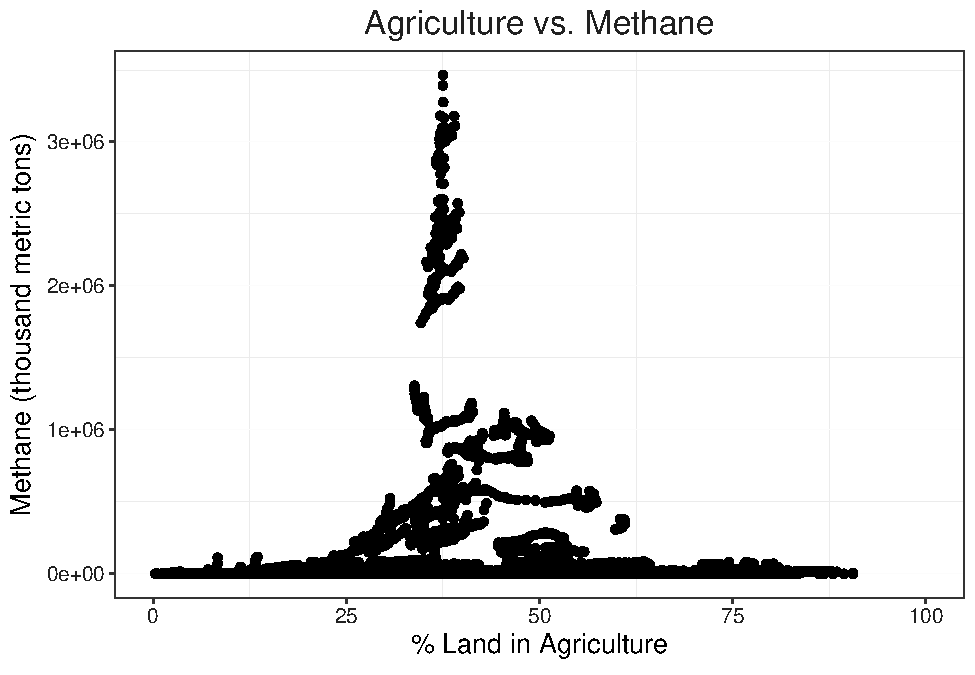
\includegraphics{Marx_ENV872_Project_files/figure-latex/unnamed-chunk-4-1.pdf}

\begin{Shaded}
\begin{Highlighting}[]
\NormalTok{LegendTitle1 <-}\StringTok{"Land Use"}

\NormalTok{FourCountries.Facet <-}\StringTok{ }
\StringTok{  }\KeywordTok{ggplot}\NormalTok{(Four_Countries) }\OperatorTok{+}
\StringTok{  }\KeywordTok{geom_line}\NormalTok{(}\KeywordTok{aes}\NormalTok{(}\DataTypeTok{x =}\NormalTok{ Year, }\DataTypeTok{y =}\NormalTok{ Agriculture, }\DataTypeTok{color =} \StringTok{"Agriculture"}\NormalTok{)) }\OperatorTok{+}\StringTok{ }
\StringTok{  }\KeywordTok{geom_line}\NormalTok{(}\KeywordTok{aes}\NormalTok{(}\DataTypeTok{x =}\NormalTok{ Year, }\DataTypeTok{y =}\NormalTok{ Forest, }\DataTypeTok{color =} \StringTok{"Forest"}\NormalTok{)) }\OperatorTok{+}\StringTok{ }
\StringTok{  }\KeywordTok{facet_grid}\NormalTok{(}\DataTypeTok{rows =} \KeywordTok{vars}\NormalTok{(Country)) }\OperatorTok{+}
\StringTok{  }\KeywordTok{ggtitle}\NormalTok{(}\StringTok{"Change in Land Use"}\NormalTok{) }\OperatorTok{+}
\StringTok{  }\KeywordTok{ylab}\NormalTok{(}\KeywordTok{expression}\NormalTok{(}\StringTok{"Land Area (%)"}\NormalTok{)) }\OperatorTok{+}
\StringTok{  }\KeywordTok{scale_x_date}\NormalTok{(}\DataTypeTok{limits =} \KeywordTok{as.Date}\NormalTok{(}\KeywordTok{c}\NormalTok{(}\StringTok{"1990-04-09"}\NormalTok{, }\StringTok{"2014-04-09"}\NormalTok{)),}
  \DataTypeTok{date_breaks =} \StringTok{"24 months"}\NormalTok{, }\DataTypeTok{date_labels =} \StringTok{"%Y"}\NormalTok{) }\OperatorTok{+}
\StringTok{  }\KeywordTok{scale_y_continuous}\NormalTok{(}\DataTypeTok{limits =} \KeywordTok{c}\NormalTok{(}\DecValTok{0}\NormalTok{,}\DecValTok{70}\NormalTok{)) }\OperatorTok{+}
\StringTok{  }\KeywordTok{scale_color_manual}\NormalTok{(LegendTitle1,}\DataTypeTok{values =} \KeywordTok{c}\NormalTok{(}\StringTok{"gold3"}\NormalTok{, }\StringTok{"darkcyan"}\NormalTok{)) }\OperatorTok{+}
\StringTok{  }\KeywordTok{labs}\NormalTok{(}\DataTypeTok{caption =} \StringTok{"Data Source: World Bank"}\NormalTok{)}
\KeywordTok{print}\NormalTok{(FourCountries.Facet)}
\end{Highlighting}
\end{Shaded}

\begin{verbatim}
## Warning: Removed 35 rows containing missing values (geom_path).

## Warning: Removed 35 rows containing missing values (geom_path).
\end{verbatim}

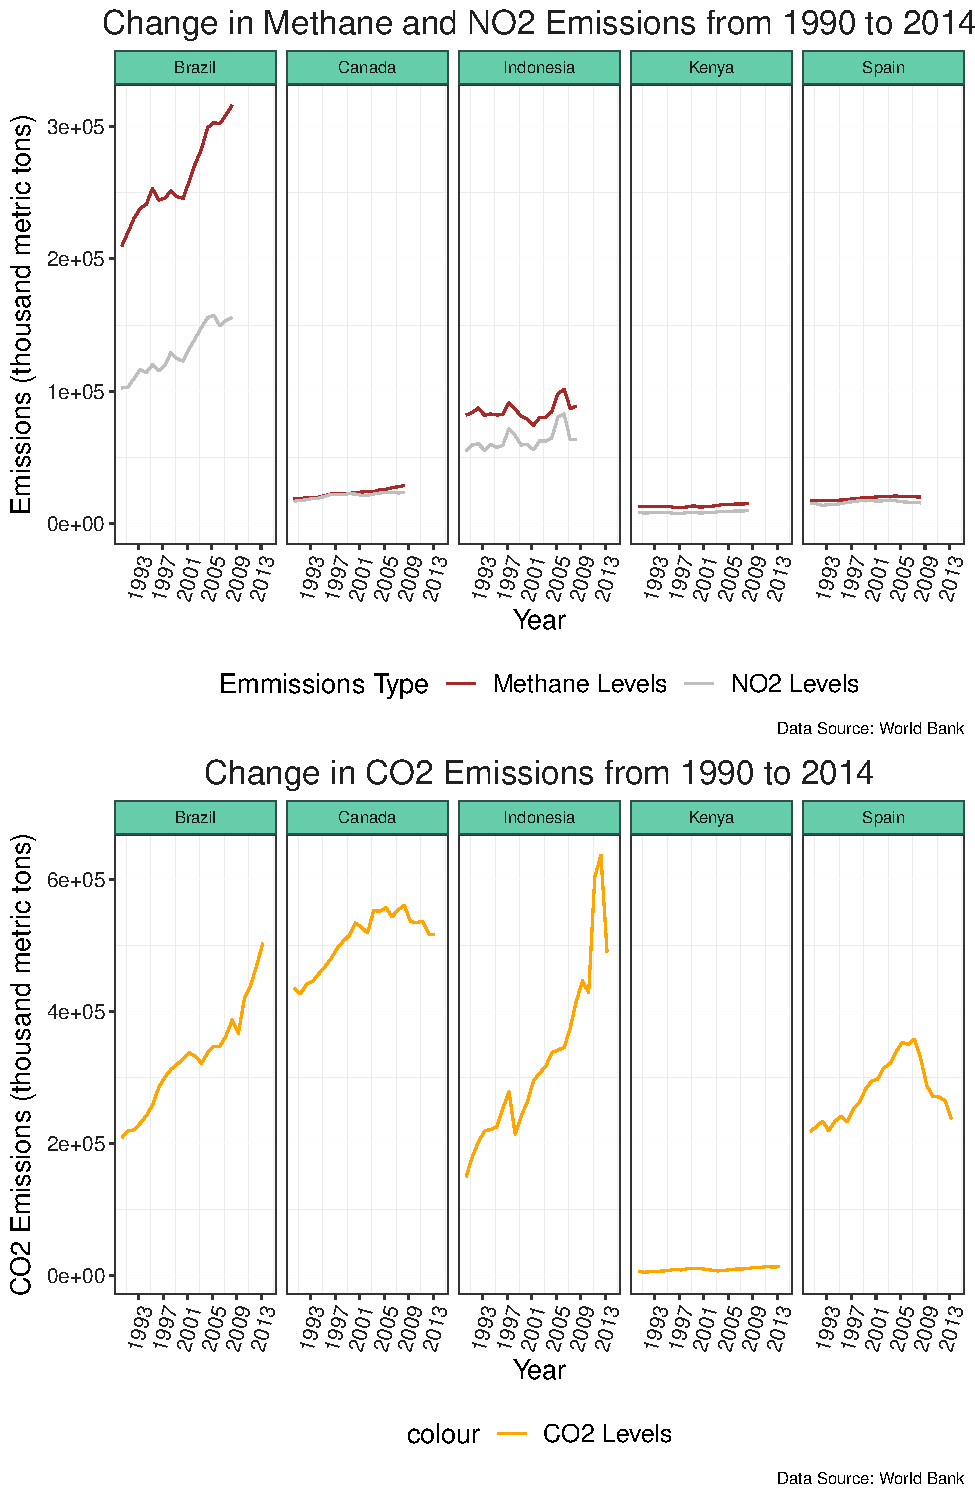
\includegraphics{Marx_ENV872_Project_files/figure-latex/unnamed-chunk-5-1.pdf}

\begin{Shaded}
\begin{Highlighting}[]
\NormalTok{FiveCountries.Facet <-}\StringTok{ }
\StringTok{  }\KeywordTok{ggplot}\NormalTok{(Five_Countries) }\OperatorTok{+}
\StringTok{  }\KeywordTok{geom_line}\NormalTok{(}\KeywordTok{aes}\NormalTok{(}\DataTypeTok{x =}\NormalTok{ Year, }\DataTypeTok{y =}\NormalTok{ Agriculture, }\DataTypeTok{color =} \StringTok{"Agriculture"}\NormalTok{)) }\OperatorTok{+}\StringTok{ }
\StringTok{  }\KeywordTok{geom_line}\NormalTok{(}\KeywordTok{aes}\NormalTok{(}\DataTypeTok{x =}\NormalTok{ Year, }\DataTypeTok{y =}\NormalTok{ Forest, }\DataTypeTok{color =} \StringTok{"Forest"}\NormalTok{)) }\OperatorTok{+}\StringTok{ }
\StringTok{  }\KeywordTok{facet_grid}\NormalTok{(}\DataTypeTok{rows =} \KeywordTok{vars}\NormalTok{(Country)) }\OperatorTok{+}
\StringTok{  }\KeywordTok{ggtitle}\NormalTok{(}\StringTok{"Change in Land Use from 1990 to 2014"}\NormalTok{) }\OperatorTok{+}
\StringTok{  }\KeywordTok{ylab}\NormalTok{(}\KeywordTok{expression}\NormalTok{(}\StringTok{"Land Area (%)"}\NormalTok{)) }\OperatorTok{+}
\StringTok{  }\KeywordTok{scale_x_date}\NormalTok{(}\DataTypeTok{limits =} \KeywordTok{as.Date}\NormalTok{(}\KeywordTok{c}\NormalTok{(}\StringTok{"1990-04-09"}\NormalTok{, }\StringTok{"2014-04-09"}\NormalTok{)),}
  \DataTypeTok{date_breaks =} \StringTok{"24 months"}\NormalTok{, }\DataTypeTok{date_labels =} \StringTok{"%Y"}\NormalTok{) }\OperatorTok{+}
\StringTok{  }\KeywordTok{scale_y_continuous}\NormalTok{(}\DataTypeTok{limits =} \KeywordTok{c}\NormalTok{(}\DecValTok{0}\NormalTok{,}\DecValTok{70}\NormalTok{)) }\OperatorTok{+}
\StringTok{  }\KeywordTok{scale_color_manual}\NormalTok{(LegendTitle1,}\DataTypeTok{values =} \KeywordTok{c}\NormalTok{(}\StringTok{"goldenrod3"}\NormalTok{, }\StringTok{"darkcyan"}\NormalTok{)) }\OperatorTok{+}
\StringTok{  }\KeywordTok{labs}\NormalTok{(}\DataTypeTok{caption =} \StringTok{"Data Source: World Bank"}\NormalTok{) }\OperatorTok{+}
\StringTok{  }\KeywordTok{theme}\NormalTok{(}\DataTypeTok{strip.background =} \KeywordTok{element_rect}\NormalTok{(}\DataTypeTok{fill=} \StringTok{"aquamarine3"}\NormalTok{, }\StringTok{"darkslategray"}\NormalTok{)) }
\KeywordTok{print}\NormalTok{(FiveCountries.Facet)}
\end{Highlighting}
\end{Shaded}

\begin{verbatim}
## Warning: Removed 35 rows containing missing values (geom_path).

## Warning: Removed 35 rows containing missing values (geom_path).
\end{verbatim}

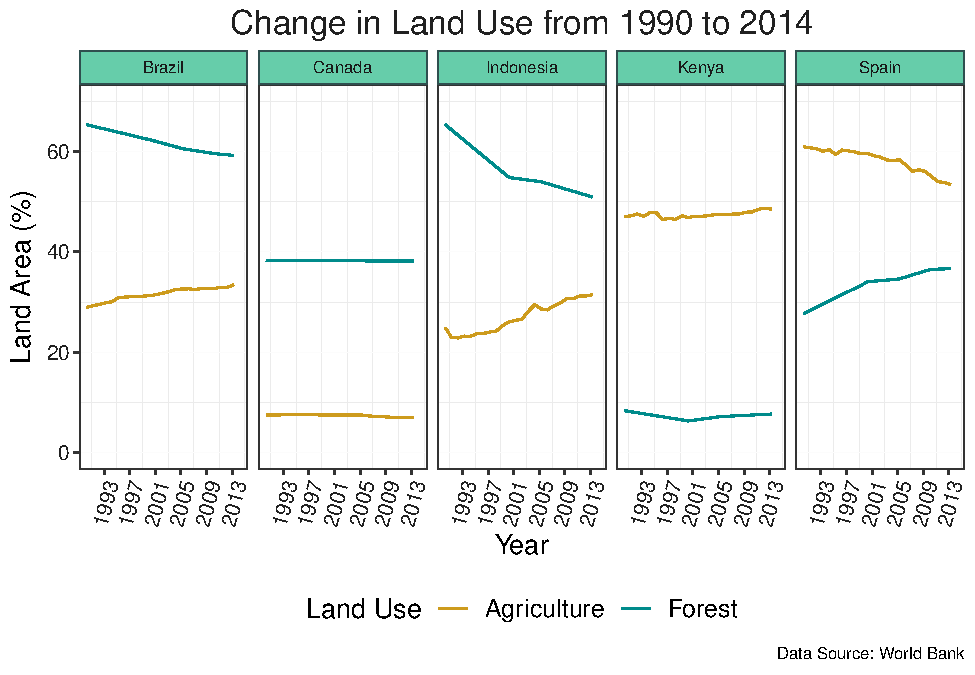
\includegraphics{Marx_ENV872_Project_files/figure-latex/unnamed-chunk-6-1.pdf}

\begin{Shaded}
\begin{Highlighting}[]
\CommentTok{#seashell3 turquoise palegreen3 darkseagreen3 darkcyan aquamarine3}
\end{Highlighting}
\end{Shaded}

\begin{Shaded}
\begin{Highlighting}[]
\NormalTok{SixCountries.Facet <-}\StringTok{ }
\StringTok{  }\KeywordTok{ggplot}\NormalTok{(Six_Countries) }\OperatorTok{+}
\StringTok{  }\KeywordTok{geom_line}\NormalTok{(}\KeywordTok{aes}\NormalTok{(}\DataTypeTok{x =}\NormalTok{ Year, }\DataTypeTok{y =}\NormalTok{ Agriculture, }\DataTypeTok{color =} \StringTok{"Agriculture"}\NormalTok{)) }\OperatorTok{+}\StringTok{ }
\StringTok{  }\KeywordTok{geom_line}\NormalTok{(}\KeywordTok{aes}\NormalTok{(}\DataTypeTok{x =}\NormalTok{ Year, }\DataTypeTok{y =}\NormalTok{ Forest, }\DataTypeTok{color =} \StringTok{"Forest"}\NormalTok{)) }\OperatorTok{+}\StringTok{ }
\StringTok{  }\KeywordTok{facet_grid}\NormalTok{(}\DataTypeTok{rows =} \KeywordTok{vars}\NormalTok{(Country)) }\OperatorTok{+}
\StringTok{  }\KeywordTok{ggtitle}\NormalTok{(}\StringTok{"Change in Land Use"}\NormalTok{) }\OperatorTok{+}
\StringTok{  }\KeywordTok{ylab}\NormalTok{(}\KeywordTok{expression}\NormalTok{(}\StringTok{"Land Area (%)"}\NormalTok{)) }\OperatorTok{+}
\StringTok{  }\KeywordTok{scale_x_date}\NormalTok{(}\DataTypeTok{limits =} \KeywordTok{as.Date}\NormalTok{(}\KeywordTok{c}\NormalTok{(}\StringTok{"1990-04-09"}\NormalTok{, }\StringTok{"2014-04-09"}\NormalTok{)),}
  \DataTypeTok{date_breaks =} \StringTok{"24 months"}\NormalTok{, }\DataTypeTok{date_labels =} \StringTok{"%Y"}\NormalTok{) }\OperatorTok{+}
\StringTok{  }\KeywordTok{scale_y_continuous}\NormalTok{(}\DataTypeTok{limits =} \KeywordTok{c}\NormalTok{(}\DecValTok{0}\NormalTok{,}\DecValTok{65}\NormalTok{)) }\OperatorTok{+}
\StringTok{  }\KeywordTok{scale_color_manual}\NormalTok{(LegendTitle1,}\DataTypeTok{values =} \KeywordTok{c}\NormalTok{(}\StringTok{"goldenrod3"}\NormalTok{, }\StringTok{"darkcyan"}\NormalTok{)) }\OperatorTok{+}
\StringTok{  }\KeywordTok{labs}\NormalTok{(}\DataTypeTok{caption =} \StringTok{"Data Source: World Bank"}\NormalTok{) }\OperatorTok{+}
\StringTok{  }\KeywordTok{theme}\NormalTok{(}\DataTypeTok{strip.background =} \KeywordTok{element_rect}\NormalTok{(}\DataTypeTok{fill=} \StringTok{"ivory2"}\NormalTok{, }\StringTok{"darkslategray"}\NormalTok{))}
\KeywordTok{print}\NormalTok{(SixCountries.Facet)}
\end{Highlighting}
\end{Shaded}

\begin{verbatim}
## Warning: Removed 35 rows containing missing values (geom_path).
\end{verbatim}

\begin{verbatim}
## Warning: Removed 37 rows containing missing values (geom_path).
\end{verbatim}

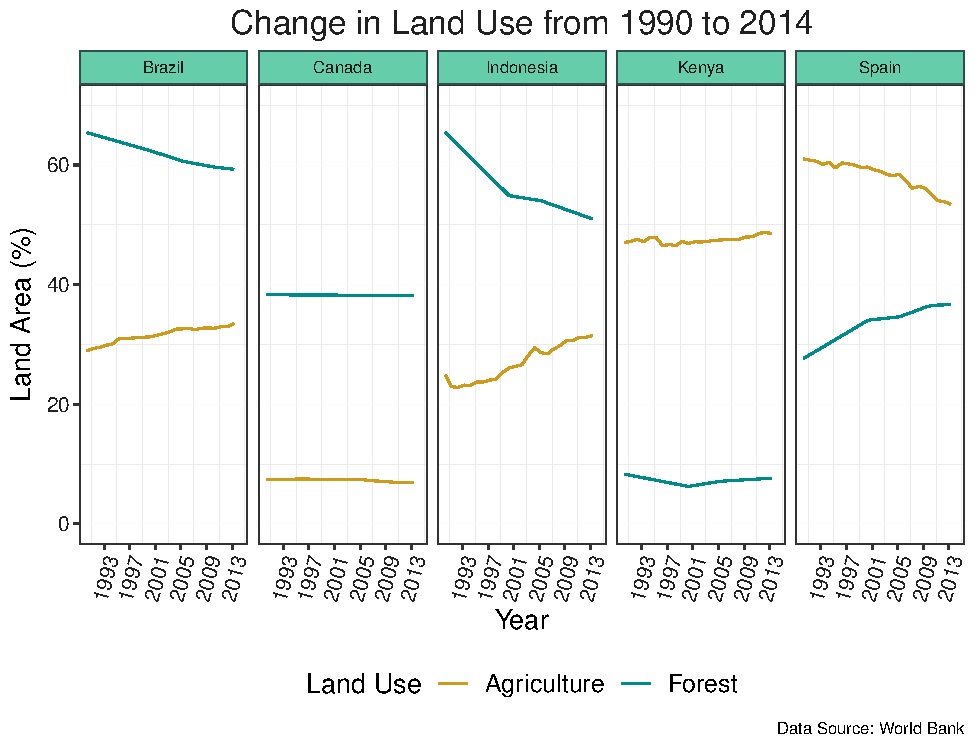
\includegraphics{Marx_ENV872_Project_files/figure-latex/unnamed-chunk-7-1.pdf}

\begin{Shaded}
\begin{Highlighting}[]
\CommentTok{#Plot1}
\NormalTok{RenewableElectricity <-}\StringTok{ }
\StringTok{  }\KeywordTok{ggplot}\NormalTok{(Four_Countries) }\OperatorTok{+}
\StringTok{  }\KeywordTok{geom_line}\NormalTok{(}\KeywordTok{aes}\NormalTok{(}\DataTypeTok{x =}\NormalTok{ Year, }\DataTypeTok{y =}\NormalTok{ RenewableElectricity)) }\OperatorTok{+}\StringTok{ }
\StringTok{  }\KeywordTok{facet_grid}\NormalTok{(}\DataTypeTok{rows =} \KeywordTok{vars}\NormalTok{(Country)) }\OperatorTok{+}
\StringTok{  }\KeywordTok{ggtitle}\NormalTok{(}\StringTok{"Renewable Electricity Output"}\NormalTok{) }\OperatorTok{+}
\StringTok{  }\KeywordTok{ylab}\NormalTok{(}\KeywordTok{expression}\NormalTok{(}\StringTok{"% of Total Electricity Output"}\NormalTok{)) }\OperatorTok{+}
\StringTok{  }\KeywordTok{scale_x_date}\NormalTok{(}\DataTypeTok{limits =} \KeywordTok{as.Date}\NormalTok{(}\KeywordTok{c}\NormalTok{(}\StringTok{"1990-04-09"}\NormalTok{, }\StringTok{"2014-04-09"}\NormalTok{)),}
  \DataTypeTok{date_breaks =} \StringTok{"24 months"}\NormalTok{, }\DataTypeTok{date_labels =} \StringTok{"%Y"}\NormalTok{) }\OperatorTok{+}
\StringTok{  }\KeywordTok{scale_y_continuous}\NormalTok{(}\DataTypeTok{limits =} \KeywordTok{c}\NormalTok{(}\DecValTok{0}\NormalTok{,}\DecValTok{100}\NormalTok{)) }\OperatorTok{+}
\StringTok{  }\KeywordTok{labs}\NormalTok{(}\DataTypeTok{caption =} \StringTok{"Data Source: World Bank"}\NormalTok{)}
\KeywordTok{print}\NormalTok{(RenewableElectricity)}
\end{Highlighting}
\end{Shaded}

\begin{verbatim}
## Warning: Removed 35 rows containing missing values (geom_path).
\end{verbatim}

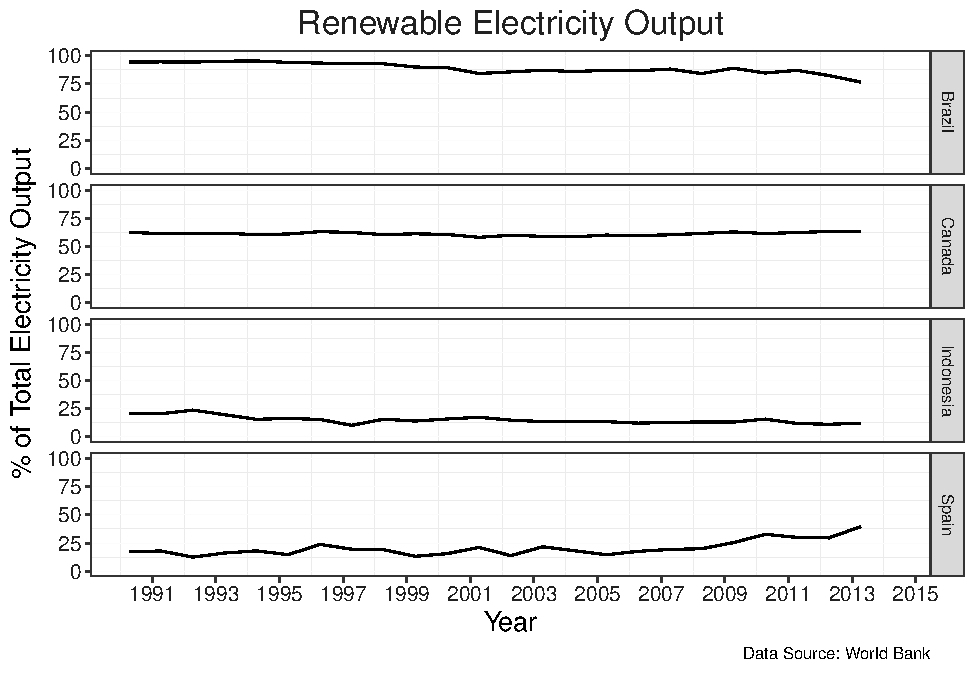
\includegraphics{Marx_ENV872_Project_files/figure-latex/unnamed-chunk-8-1.pdf}

\begin{Shaded}
\begin{Highlighting}[]
\NormalTok{RE <-}\StringTok{ }
\StringTok{  }\KeywordTok{ggplot}\NormalTok{(}\DataTypeTok{data =}\NormalTok{ Four_Countries, }\KeywordTok{aes}\NormalTok{(}\DataTypeTok{x =}\NormalTok{ Year, }\DataTypeTok{y =}\NormalTok{ RenewableElectricity, }\DataTypeTok{color =}\NormalTok{ Country)) }\OperatorTok{+}
\StringTok{  }\KeywordTok{geom_line}\NormalTok{()}\OperatorTok{+}
\StringTok{  }\KeywordTok{ggtitle}\NormalTok{(}\StringTok{"Renewable Electricity Output"}\NormalTok{) }\OperatorTok{+}
\StringTok{  }\KeywordTok{ylab}\NormalTok{(}\KeywordTok{expression}\NormalTok{(}\StringTok{"% of Total Electricity Output"}\NormalTok{)) }\OperatorTok{+}
\StringTok{  }\KeywordTok{scale_x_date}\NormalTok{(}\DataTypeTok{limits =} \KeywordTok{as.Date}\NormalTok{(}\KeywordTok{c}\NormalTok{(}\StringTok{"1990-04-09"}\NormalTok{, }\StringTok{"2014-04-09"}\NormalTok{)),}
  \DataTypeTok{date_breaks =} \StringTok{"24 months"}\NormalTok{, }\DataTypeTok{date_labels =} \StringTok{"%Y"}\NormalTok{) }\OperatorTok{+}
\StringTok{  }\KeywordTok{scale_y_continuous}\NormalTok{(}\DataTypeTok{limits =} \KeywordTok{c}\NormalTok{(}\DecValTok{0}\NormalTok{,}\DecValTok{100}\NormalTok{)) }\OperatorTok{+}
\StringTok{  }\KeywordTok{labs}\NormalTok{(}\DataTypeTok{caption =} \StringTok{"Data Source: World Bank"}\NormalTok{)}
\KeywordTok{print}\NormalTok{(RE)}
\end{Highlighting}
\end{Shaded}

\begin{verbatim}
## Warning: Removed 140 rows containing missing values (geom_path).
\end{verbatim}

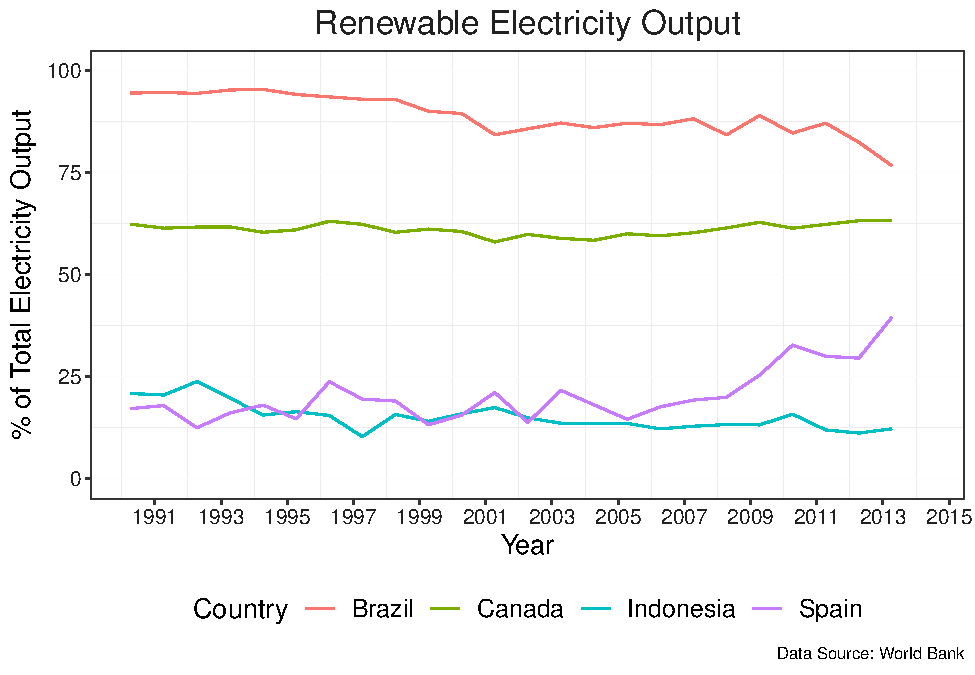
\includegraphics{Marx_ENV872_Project_files/figure-latex/unnamed-chunk-8-2.pdf}

\begin{Shaded}
\begin{Highlighting}[]
\CommentTok{# Plots}
\end{Highlighting}
\end{Shaded}

\newpage

\section{Analysis}\label{analysis}

\newpage

\section{Summary and Conclusions}\label{summary-and-conclusions}


\end{document}
